\subsubsection{Example}

    \begin{itemize}[noitemsep,topsep=0pt]
      \item Starting position: (0.0, -4.0, 32.0)
      \item End position: (0.0, -2.0, 8.0) 
      \item Euclidean distance from the object: 8.246211251235321
      \item Object can be seen: True
      \item Success: True
      \item Object type: a campsite
      
    \end{itemize}
    

    \begin{center}
    \includegraphics[width=0.7\linewidth]{images/GPT4o-ForestNew/25_r0_.pdf}
    \end{center}
    

    \begin{center}
    \includegraphics[width=0.7\linewidth]{images/GPT4o-ForestNew/25_r0__sit_awareness.pdf}
    \end{center}
    

    \begin{drama}
    \Character{Benchmark}{re}
    \Character{GPT-4o}{gpt}
    
\respeaks: \( < \)Context\( > \)
    You are in command of a UAV, tasked with finding a campsite.
\( < \)/Context\( > \) \texttt{(REST OF THE PROMPT)}
\StageDir{\re{} presents \gpt{} with a relevant image}

    \begin{center}
    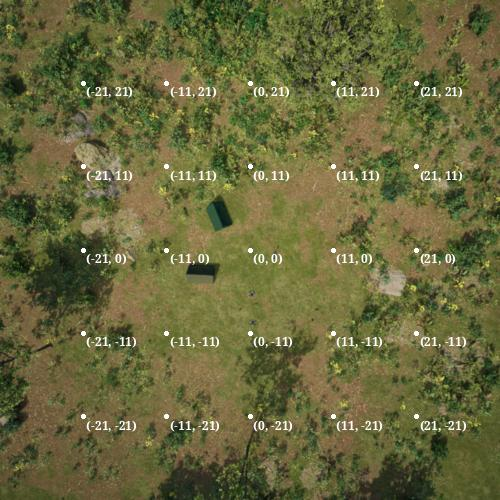
\includegraphics[width=0.5\linewidth]{images/GPT4o-ForestNew/25_r0__0.jpg}
    \end{center}
    
\respeaks: Your current altitude is 32 meters above ground level.
\gptspeaks: \( < \)Reasoning\( > \)
The two green tents in the center of the grid at (0, 0) resemble a campsite. I will descend directly to ensure I am below 10 meters above them.
\( < \)/Reasoning\( > \)
\( < \)Action\( > \)(0, 0, -24)\( < \)/Action\( > \)
\StageDir{\re{} presents \gpt{} with a relevant image}

    \begin{center}
    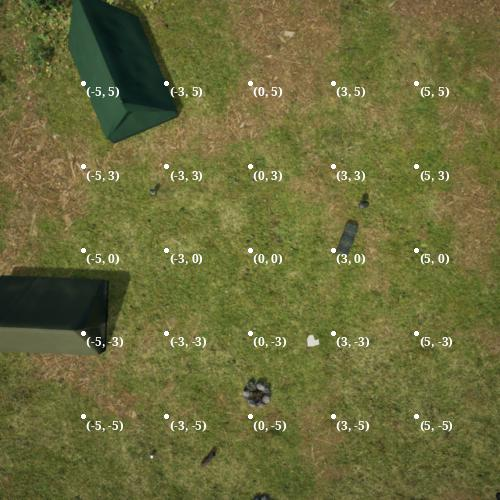
\includegraphics[width=0.5\linewidth]{images/GPT4o-ForestNew/25_r0__1.jpg}
    \end{center}
    
\respeaks: Your current altitude is 8 meters above ground level.
\gptspeaks: \( < \)Reasoning\( > \)
The two green tents at (0, 0) are clearly visible and centered. I am at 8 meters above them, which is below the required 10 meters. This is the campsite.
\( < \)/Reasoning\( > \)
\( < \)FOUND /\( > \)
\end{drama}
\subsubsection{Example}

    \begin{itemize}[noitemsep,topsep=0pt]
      \item Starting position: (7.0, -1.0, 74.0)
      \item End position: (7.0, 0.0, 8.0) 
      \item Euclidean distance from the object: 10.63014581273465
      \item Object can be seen: True
      \item Success: True
      \item Object type: a building
      
    \end{itemize}
    

    \begin{center}
    \includegraphics[width=0.7\linewidth]{images/GPT4o-ForestNew/27_r0_.pdf}
    \end{center}
    

    \begin{center}
    \includegraphics[width=0.7\linewidth]{images/GPT4o-ForestNew/27_r0__sit_awareness.pdf}
    \end{center}
    

    \begin{drama}
    \Character{Benchmark}{re}
    \Character{GPT-4o}{gpt}
    
\respeaks: \( < \)Context\( > \)
    You are in command of a UAV, tasked with finding a building.
\( < \)/Context\( > \) \texttt{(REST OF THE PROMPT)}
\StageDir{\re{} presents \gpt{} with a relevant image}

    \begin{center}
    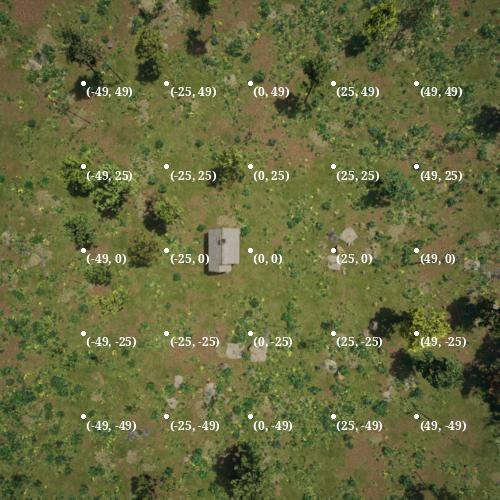
\includegraphics[width=0.5\linewidth]{images/GPT4o-ForestNew/27_r0__0.jpg}
    \end{center}
    
\respeaks: Your current altitude is 74 meters above ground level.
\gptspeaks: \( < \)Reasoning\( > \)The building is clearly visible at the center of the grid. I will lower the altitude to get within the required 10 meters above the building to confirm the objective.\( < \)/Reasoning\( > \)
\( < \)Action\( > \)(0, 0, -65)\( < \)/Action\( > \)
\StageDir{\re{} presents \gpt{} with a relevant image}

    \begin{center}
    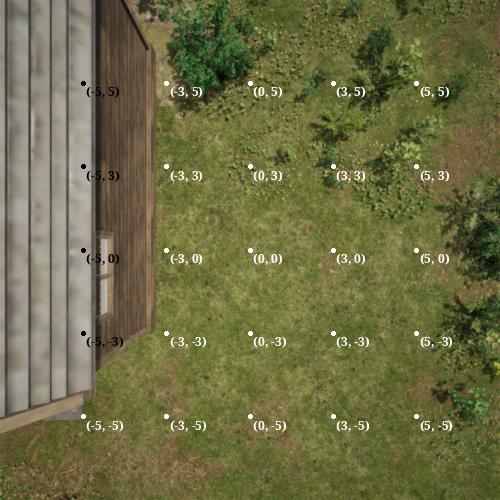
\includegraphics[width=0.5\linewidth]{images/GPT4o-ForestNew/27_r0__1.jpg}
    \end{center}
    
\respeaks: Your current altitude is 8 meters above ground level.
\gptspeaks: \( < \)Reasoning\( > \)The building is now in view and I am within 10 meters above it. I will confirm the objective.\( < \)/Reasoning\( > \)
\( < \)Action\( > \)FOUND\( < \)/Action\( > \)
\end{drama}
